\chapter{Проектирование информационной системы «Личный кабинет абитуриента»}

\section{Проектирование архитектуры веб-приложения}

Перед началом проектирования архитектуры веб-приложения, следует выбрать какой тип архитектуры использовать. Существует множество различных подходов проектирования архитектуры веб-приложений, самые популярные на текущий момент это микросервисная архитектура и монолитная архитектура, которая, как правило, представляет собой веб-приложение с 3-х уровневой архитектурой \cite{webapacrch}.

Монолитная архитектура является традиционным методом разработки веб-приложений. Монолитное приложение полностью замкнуто в контексте поведения. Во время работы оно может взаимодействовать с другими службами или хранилищами данных, однако основа его поведения реализуется в собственном процессе, а все приложение обычно развертывается как один элемент (рисунок \ref{fig:monolit}). Для горизонтального масштабирования такое приложение обычно целиком дублируется на нескольких серверах или виртуальных машинах \cite{monolith}. Как правило, такие приложения состоят из следующих слоев:

\begin{enumerate} 
  \item слой представления — содержит пользовательский интерфейс и отвечает за обеспечение хорошего пользовательского опыта;
  
  \item слой бизнес-логики — отделяет пользовательский интерфейс от вычислений, связанных с бизнесом;
  
  \item слой передачи данных — отвечает за взаимодействие с постоянными хранилищами, такими как базы данных, и прочую обработку информации, которая не связана с бизнесом.
\end{enumerate}

\begin{figure}[H]
\begin{center}
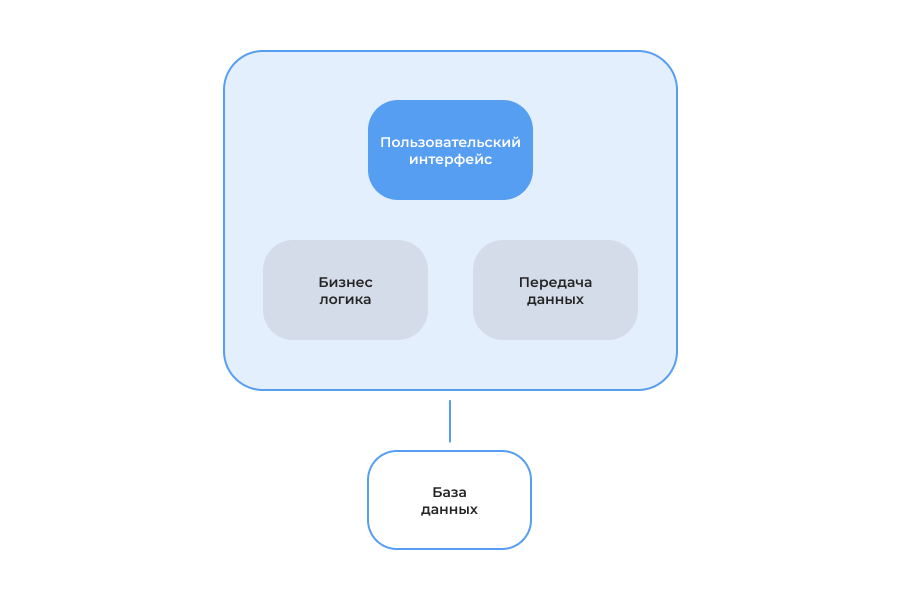
\includegraphics[width=0.9\hsize]{fig/monolit.png}\\[2mm]
\caption{Архитектура монолитного приложения из трех слоев}\label{fig:monolit}
\end{center}
\end{figure}

Преимущества монолитной архитектуры:

\begin{enumerate} 
  \item упрощенная разработка и развертывание — благодаря монолитному ядру все изменения и обновления развертываются вместе;
  
  \item быстрая связь между программными компонентами благодаря общему коду и памяти.
\end{enumerate}

Недостатки монолитной архитектуры:

\begin{enumerate} 
  \item утяжеление кодовой базы — с течение времени, кодовая база монолитных веб-приложений становится трудной для понимания и изменения;
  
  \item слабая гибкость — любое небольшое изменение требует повторного развертывания всего веб-приложения;
  
  \item сильная связанность — ошибка в одном из модулей веб-приложения способна разрушить все веб-приложение целиком.
\end{enumerate}

Микросервисная архитектура представляет собой множество слабо связанных сервисов, взаимодействующих друг с другом для выполнения задач (рисунок \ref{fig:microservices}). Каждый такой сервис максимально автономен, необходим для выполнения конкретной задачи и может поддерживаться отдельной командой разработчиков. Данная архитектура позволяет применять модульный принцип построения веб-приложения \cite{microservice}.

\begin{figure}[H]
\begin{center}
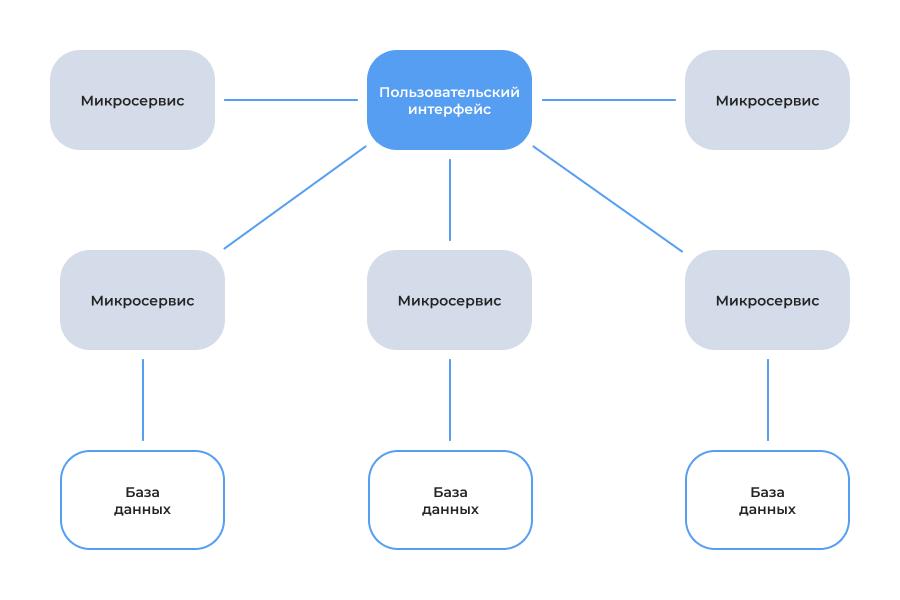
\includegraphics[width=0.9\hsize]{fig/microservices.png}\\[2mm]
\caption{Микросервисная архитектура}\label{fig:microservices}
\end{center}
\end{figure}

Преимущества микросервисной архитектуры:

\begin{enumerate} 
  \item слабая связанность — благодаря высокой степени изоляции, сбой в одном сервисе не затронет систему в целом;
  
  \item высокая степень масштабируемости — каждый сервис может разрабатываться, внедряться и масштабироваться по отдельности;
  
  \item разделение кодовых баз — каждый сервис имеет отдельную кодовую базу и может быть разработан с использованием разных языков программирования.
\end{enumerate}

Недостатки микросервисной архитектуры:

\begin{enumerate} 
  \item высокие требования к скорости канала между сервисами;
  
  \item сложность реализации взаимодействия между сервисами и их комплексном тестировании.
\end{enumerate}

Для реализации информационной системы «Личный кабинет абитуриента» выбрана микросервисная архитектура, благодаря которой, разработка клиентской и серверной части может вестись параллельно, а функционал информационной системы может быть легко расширен путем подключения новых сервисов.

На текущий момент, реализовано одностраничное веб-приложение, сервис REST-API для личного кабинет абитуриента, база данных, хранящая данные личного кабинета абитуриента, сервис обновления справочников, интеграция с системой учета «1С Университет», сервис резервного копирования, файловая система, сервис REST-API ФИАС, база данных, хранящая сведения об адресах, сервис обновления данных ФИАС. Общую конфигурацию и топологию информационной системы можно увидеть на диаграмме развертывания (рисунок \ref{fig:diagramdeploy}).

\begin{figure}[H]
\begin{center}
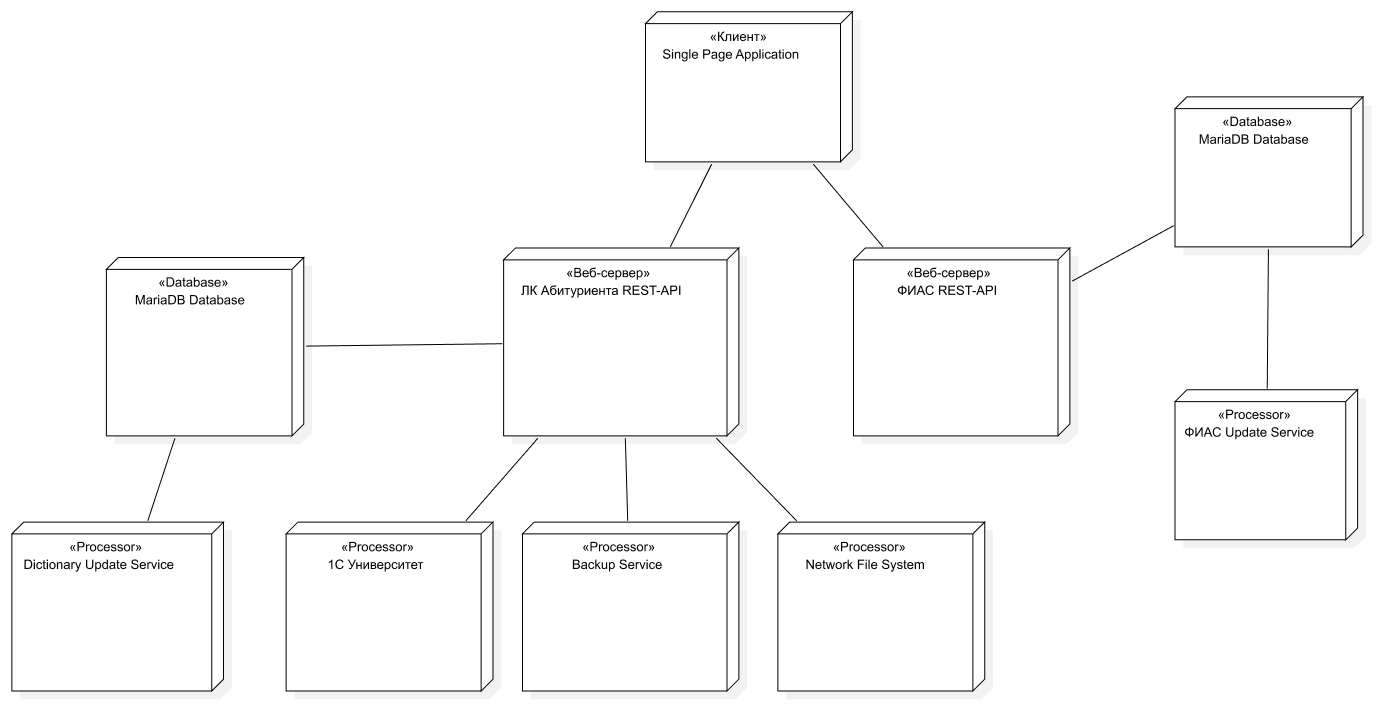
\includegraphics[width=1\hsize]{fig/diagram-deploy.png}\\[2mm]
\caption{Диаграмма развертывания информационной системы «Личный кабинет абитуриента»}\label{fig:diagramdeploy}
\end{center}
\end{figure}

Клиентская часть информационной системы будет реализована в виде одностраничного приложения. Single page application (SPA) — одностраничное веб-приложение, загружающие одну HTML-страницу и благодаря динамическому обновлению с помощью AJAX запросов, загружает данные и дополнительные страницы. Данные подход позволяет реализовать гибкий и отзывчивый интерфейс, поскольку все необходимые ресурсы загружаются без перезагрузки веб-страницы \cite{spa}.

\section{Проектирование пользовательского интерфейса}

Перед началом реализации клиентской части информационной системы, необходимо спроектировать все основные шаблоны веб-приложения, а также те части веб-приложения, интерфейс которых требует предварительного согласования.

Шаблоном в одностраничных приложениях называется компонент, который содержит в себе некоторые повторяющиеся на разных страницах элементы, а также основную часть, которая меняется на разных страницах \cite{designinfsystems}.

В веб-приложении «Личный кабинет абитуриента» будет использоваться два шаблона.

Шаблон для представлений авторизация (рисунок \ref{fig:templateauth}), регистрация (рисунок \ref{fig:templatereg}), восстановления пароля, будет содержать в себе шапку, место для основного содержимого страницы и подвал.

\begin{figure}[H]
\begin{center}
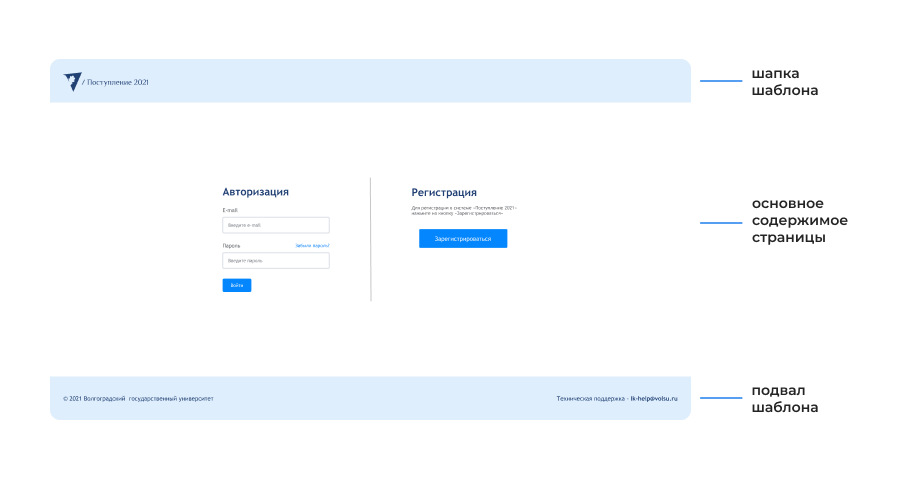
\includegraphics[width=1\hsize]{fig/template.png}\\[2mm]
\caption{Спроектированный шаблон для представления авторизация}\label{fig:templateauth}
\end{center}
\end{figure}


\begin{figure}[H]
\begin{center}
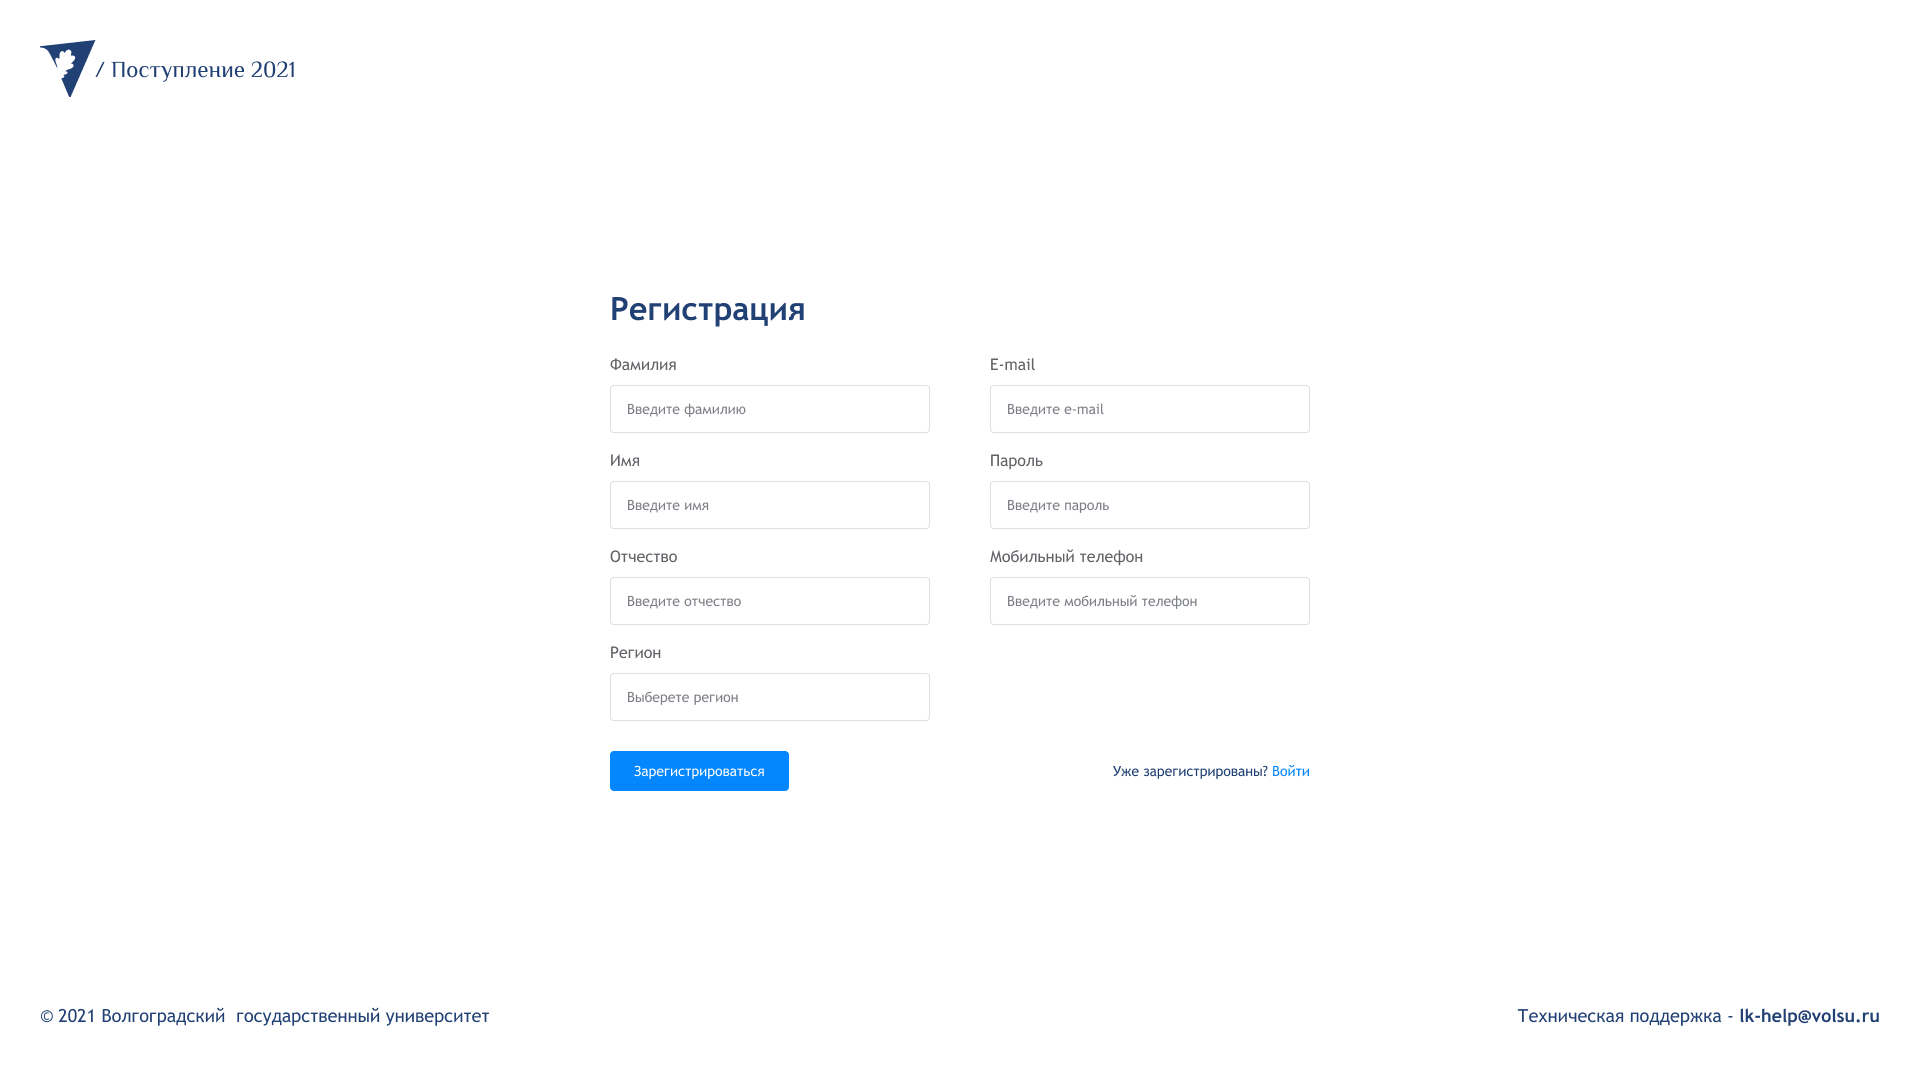
\includegraphics[width=1\hsize]{fig/template-reg.png}\\[2mm]
\caption{Спроектированный шаблон для представления регистрация}\label{fig:templatereg}
\end{center}
\end{figure}

Основной шаблон, используемый для внутренних страниц личного кабинета, содержит в себе навигационное меню и часть для основного содержимого страницы (рисунок \ref{fig:templatemain}).

\begin{figure}[H]
\begin{center}
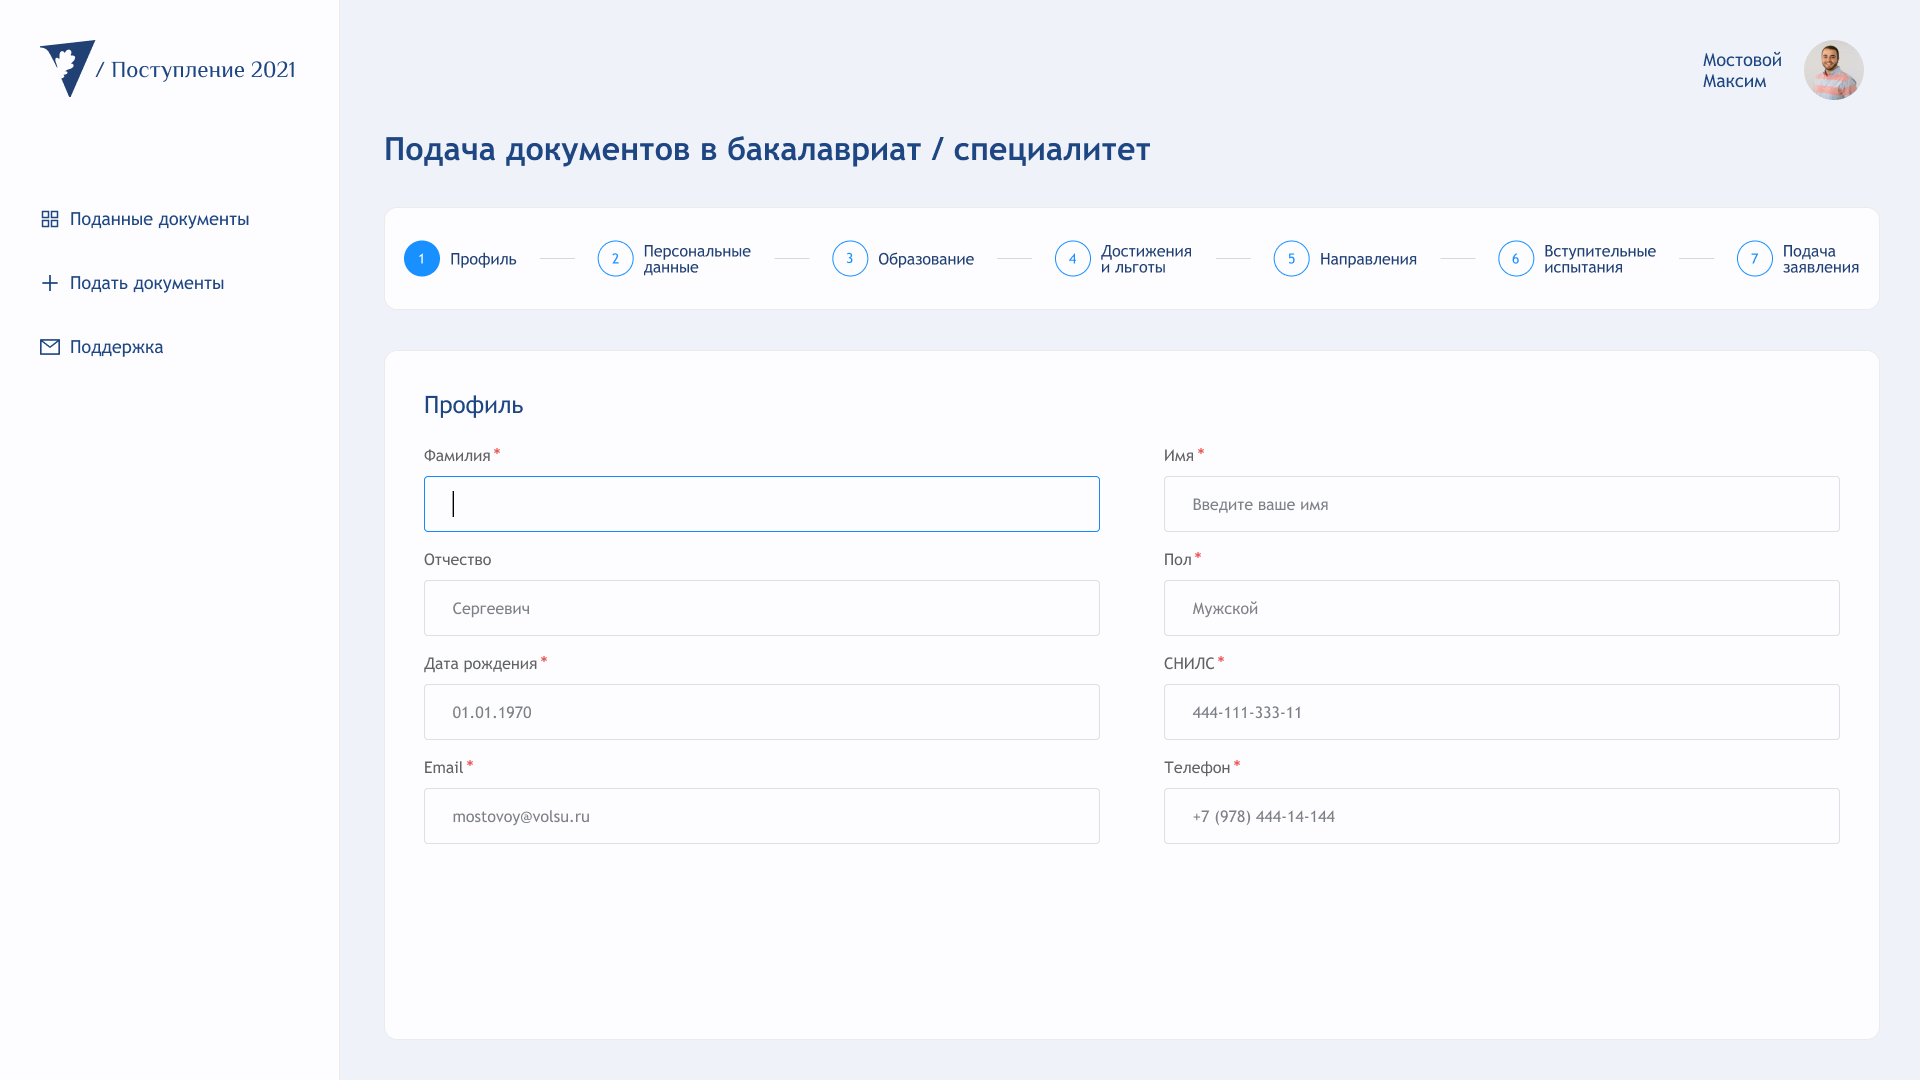
\includegraphics[width=1\hsize]{fig/main-layout-design.png}\\[2mm]
\caption{Спроектированный шаблон для внутренних страниц личного кабинета}\label{fig:templatemain}
\end{center}
\end{figure}
